\documentclass[11pt,a4paper]{article}
\usepackage[utf8]{inputenc}
\usepackage{amsmath,enumitem,amsfonts,amssymb,graphicx,commath}
\usepackage{sectsty}
\usepackage{multicol}
\usepackage{tikz}

\graphicspath{ {./img/} }
\DeclareMathAlphabet{\pazocal}{OMS}{zplm}{m}{n}
\usetikzlibrary{arrows,automata}

\usepackage[%
    left=1in,%
    right=1.0in,%
    top=0.8in,%
    bottom=1in,%
]{geometry}%

\sectionfont
{\fontsize{14.4}{12}\selectfont}
\title{\textbf{Principles of AI Planning
		\\{\Large Exercise Sheet 9}}}
\makeatletter
\renewcommand{\@maketitle}
{
	\newpage
	\null
	\vskip 2em%
	\begin{center}%
		{\LARGE \@title \\ \par}%
	\end{center}%
	\par
} \makeatother

\begin{document}
\begin{flushleft}
	Authors:\\
	Erick Rosete Beas | er165@uni-freiburg.de\\
	Jessica Lizeth Borja Diaz | jb986@uni-freiburg.de\\
\end{flushleft}
{\let\newpage\relax\maketitle}
\begin{center} 
	\large 10.01.2020
\end{center}


%%%%%%%%%%%%%%%%%%%%%  Ejercicio 1 %%%%%%%%%%%%%%%%%%%%%%%%%
\section*{Exercise 9.1 - Additive patterns and canonical heuristic}

\begin{enumerate}[label=(\alph*), listparindent=1.5em]
	\item \textbf{Specify the compatibility graph of $\pazocal{C}$ and
	determine its maximal cliques}\\
	\textbf{Process}:\\
	To determine the compatibility graph, first we avoid drawing connections with the patterns with the same variables.\\
	$\{ P_1, P_3, P_8 \}$ share variable $at$-$goal_{s2}$\\
	$\{ P_2, P_4, P_6, P_7, P_{10} \}$ share variable $at$-$goal_{s1}$\\
	$\{ P_2, P_4\}$ share variable $position_{s1}$\\
	$\{ P_4, P_5\}$ share variable $position_{p}$\\\\
	Then we analyzed which operations affect two variables in different patterns and we find the followings:
	\begin{itemize}
		\item $move$ always affects $position_p$ but it can also affect $content_x = nothing$ to $content_x := p$ or viceversa, therefore $\{ P_4, P_5 \}$ are not orthogonal with $\{P_6, P_7, P_8, P_9, P_9, P_{10}\}$ (no line from first set to second set)
		\item $push$ affects $position_p$ and $position_{s1}$ or $position_{s2}$, therefore $\{ P_4, P_5 \}$ are not orthogonal with $\{P_2, P_3\}$
		\item $push$ affects $position_{s1}$ and $content_x$, analogously with $position_{s2}$ therefore $\{ P_2, P_3, P_4, P_5\}$ are not orthogonal with $\{P_6, P_7, P_8, P_9, P_10\}$
		\item When we $push$ box $s1$ to the goal, $position_{s1}$, $position_p$ and $at$-$goal_{s1}$ are affected, analogously with $s2$, therefore:
			\begin{itemize}
				\item $\{ P_2, P_4, P_5 \}$ are not orthogonal with $\{P_2, P_4, P_6, P_7, P_{10}\}$ because of $position_{s1}$ and $at$-$goal_{s1}$
				\item $\{ P_3\}$ are not orthogonal with $\{P_1, P_3, P_8\}$ because of $position_{s2}$ and $at$-$goal_{s2}$
				\item $\{ P_4, P_5\}$ are not orthogonal with $\{P_1, P_2, P_3, P_4, P_6, P_7, P_8, P_{10}\}$ because of $position_{p}$ and $at$-$goal_{s1}$ or $at$-$goal_{s2}$
			\end{itemize}
		\item We can $push$ a box from $Q$ to a goal position, therefore, affecting $content_Q$ and $at$-$goal_{s1}$ or $at$-$goal_{s2}$, therefore $\{ P_{10}\}$ are not orthogonal with $\{P_1, P_2, P_3, P_4, P_6, P_7, P_8\}$
		\item We can $push$ a box from $K$ to $Q$ with the agent position in $E$, $content_E$ and $content_Q$ are affected, therefore $\{ P_9\}$ and $\{P_{10}\}$ are not orthogonal.
		\item We can $push$ a box from $F$ to $E$ with the agent position in $G$, $content_G$ and $content_E$ are affected, therefore $\{ P_7\}$ and $\{P_9\}$ are not orthogonal.
		\item We can $move$ between $D$ and $E$, affecting $content_D$ and $content_E$, therefore $\{ P_8\}$ and $\{P_9\}$ are not orthogonal.
		\item We can $move$ between $G$ and $H$, affecting $content_G$ and $content_H$, therefore $\{ P_6\}$ and $\{P_7\}$ are not orthogonal.
	\end{itemize}
	
	\pagebreak
	Finally we connect the orthogonal abstractions to find the maximal cliques:\\
	\begin{center}
		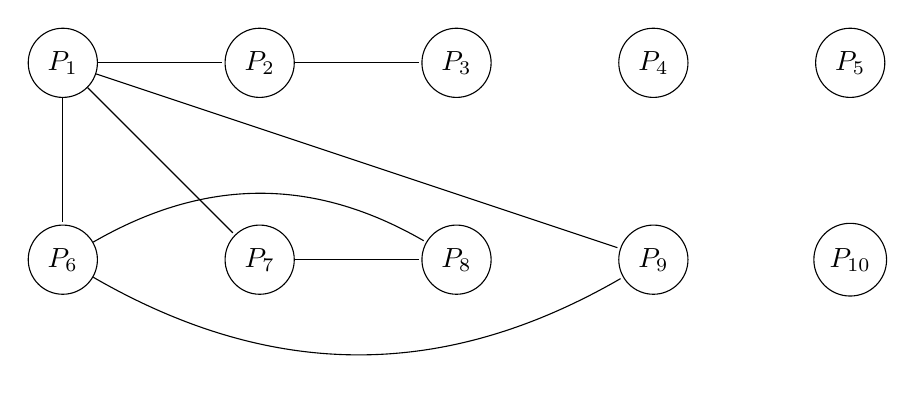
\begin{tikzpicture}[-,>=stealth',shorten >=1pt,auto,node distance=2.5cm,
		scale = 1,transform shape]
		
		\node[state] (p1) {$P_{1}$};
		\node[state] (p2) [right of=p1] {$P_{2}$};
		\node[state] (p3) [right  of=p2] {$P_{3}$};
		\node[state] (p4) [right of=p3] {$P_{4}$};
		\node[state] (p5) [right of=p4] {$P_{5}$};

		\node[state] (p6) [below  of=p1] {$P_{6}$};
		\node[state] (p7) [right of=p6] {$P_{7}$};
		\node[state] (p8) [right of=p7] {$P_{8}$};
		\node[state] (p9) [right of=p8] {$P_{9}$};
		\node[state] (p10) [right of=p9] {$P_{10}$};

		\path 
		(p1) edge          		 node{}(p2)
		(p1) edge          		 node{}(p6)
		(p1) edge          		 node{}(p7)
		(p1) edge          		 node{}(p9)
		(p2) edge          		 node{}(p3)
		(p6) edge[bend left]     node{}(p8)
		(p6) edge[bend right]    node{}(p9)
		(p7) edge          		 node{}(p8);
		\end{tikzpicture}
	\end{center}

	\begin{center}
		\begin{tabular}{c c c}
			 & Maximal Cliques & \\
			\hline \hline
			$\{P_1,P_2\}$ & $\{P_1, P_6, P_9\}$ & $\{P_1, P_7\}$ \\	
			$\{P_7,P_8\}$ & $\{P_6, P_8\}$ 		& $\{P_2, P_3\}$ \\
			$\{P_4\}$ 	  & $\{P_5\}$ 			& $\{P_{10}\}$
		\end{tabular}
	\end{center}
	\item \textbf{Determine the canonical heuristic $h^{\pazocal{C}}$
	and simplify it as much as possible}\\
	We will obtain the canonical heuristic value for the initial state given this patterns and maximal cliques.\\
	\begin{multicols}{3}
		\begin{tabular}{c c}
			$ i $		& $h^{P_i}$\\
			\hline\hline
			1 & 1 \\
			2 & 5 \\
			3 & 4 \\
			4 & 13\\
			5 & 0 \\
			6 & 1 \\
			7 & 1 \\
			8 & 1 \\
			9 & 0 \\
			10& 1 \\
		\end{tabular}

		\begin{tabular}{l | c}
			\multicolumn{2}{c}{Cliques heuristics} \\
			\hline \hline
			Clique & $h^{\pazocal{C}}$\\
			\hline
			$\{P_1,P_2\}$ 		& 6 \\
			$\{P_1, P_6, P_9\}$ & 2 \\
			$\{P_1, P_7\}$ 		& 2 \\
			$\{P_7,P_8\}$ 		& 2 \\
			$\{P_6, P_8\}$ 		& 2 \\
			$\{P_2, P_3\}$ 		& 9 \\
			$\{P_4\}$ 	  		& 13\\
			$\{P_5\}$ 			& 0 \\
			$\{P_{10}\}$		& 1
		\end{tabular}

		\[ h^{\pazocal{C}}=13\]
	\end{multicols}
	\item \textbf{Which patterns in $\pazocal{C}$ can be omitted and why?}
	
	$\>$ The patterns that don't include any variable from the goal 
	condition as they are in the same abstraction mapping $\alpha$ 
	that a goal statement the heuristic value will be 0, therefore 
	these pattern heuristics are not informative at all, these are 
	$P_5$ and $P_9$. \\
	
	\item \textbf{What would the canonical heuristic look like if we omitted
	those patterns before even constructing the compatibility graph}
	
	$\>$ As the canonical heuristic obtains the sum of all pattern 
	heuristics in cliques, and this pattern heuristic is always 0, 
	the resultant canonical heuristic won't change.\\
\end{enumerate}
\pagebreak
%%%%%%%%%%%%%%%%%%%%%  Ejercicio 2 %%%%%%%%%%%%%%%%%%%%%%%%%
\section*{Exercise 9.2 - Orthogonality and pairwise orthogonality}
Prove the following: $\alpha_1, ..., \alpha_n$ are orthogonal if and only if they are pairwise orthogonal.\\\\

\textbf{1) if $\alpha_1, ..., \alpha_n$ are orthogonal then 
they are pairwise orthogonal}\\

$\>$ If $\alpha_1, ..., \alpha_n$ are orthogonal, then by 
definition we know that for all transitions 
$\langle s, l, t\rangle$ of $\pazocal{T}$, 
we have $\alpha_i(s) \neq \alpha_i(t)$  for at most one 
$i \in \{1, ... , n\}$.
For the sake of contradiction, let's assume that 
$\alpha_1, ..., \alpha_n$ 
are not pairwise orthogonal, this implies that there 
is at least one abstraction mapping pair 
$\{ \alpha_j$ and $\alpha_k \ |\quad j,k \in \{1,...,n\},j \neq k \}$
which is not orthogonal. \\

$\>$This means that we have at least one transition 
$\langle s, l, t \rangle$ of $\pazocal{T}$ where 
$\alpha_j(s) \neq \alpha_j(t)$ and $\alpha_k(s) \neq \alpha_k(t)$, 
but this cannot be true because the entire system is orthogonal, 
which is a contradiction, therefore 
if the abstraction mappings are orthogonal then they are
pairwise orthogonal as well.\\\\

\textbf{2) if $\alpha_1, ..., \alpha_n$ are pairwise orthogonal then they are orthogonal}\\

$\>$ If $\alpha_1, ..., \alpha_n$ are pairwise orthogonal, then by 
definition we know that for all $j, k \in \{1, ... , n\}$ 
with $j \neq k$, mappings $\alpha_j$ and $\alpha_k$ are orthogonal.
For the sake of contradiction let's assume that the abstraction 
mappings are not orthogonal, this implies that there are at least 
two abstraction mappings
$\{ \alpha_j$ and $\alpha_k \ |\quad j,k \in \{1,...,n\},j \neq k \}$
 in the system where in one or more transitions
 $\langle s, l, t \rangle$ of $\pazocal{T}$, we have 
 $\alpha_i(s) \neq \alpha_i(t)$  for $i \in \{1, ... , n\}$.\\
 
 $\>$ Then $\alpha_j$ and $\alpha_k$ are not orthogonal, 
 but all the abstraction mappings are pairwise orthogonal, 
 which is a contradiction, therefore the if the abstraction mappings 
 are pairwise orthogonal then they are also orthogonal.\\
\end{document}